\documentclass[tikz,border=10pt]{standalone}
\usepackage{tikz}
\usepackage{fontawesome5}
\usepackage{amsmath,amssymb}
\usetikzlibrary{arrows.meta,positioning,fit,backgrounds,calc,shadows,shapes.geometric}

% Color definitions
\definecolor{lavenderDark}{RGB}{15, 44, 89}
\definecolor{lavenderDeep}{RGB}{10, 28, 58}
\definecolor{lavenderMedium}{RGB}{29, 78, 158}
\definecolor{lavenderLight}{RGB}{240, 246, 255}
\definecolor{lavenderBorder}{RGB}{180, 205, 237}
\definecolor{prismNavy}{RGB}{15, 44, 89}
\definecolor{prismBlue}{RGB}{29, 78, 158}
\definecolor{prismTeal}{RGB}{13, 148, 136}
\definecolor{prismGold}{RGB}{217, 119, 6}
\definecolor{prismDark}{RGB}{15, 23, 42}
\definecolor{statusFail}{RGB}{220, 38, 38}
\definecolor{cInput}{RGB}{241, 245, 249}
\definecolor{cStem}{RGB}{224, 242, 254}
\definecolor{cStage1}{RGB}{209, 250, 229}
\definecolor{cStage2}{RGB}{254, 243, 199}
\definecolor{cHead}{RGB}{219, 234, 254}

\begin{document}
% Complete Flowchart for Deep Learning Early Lung Disease Detection
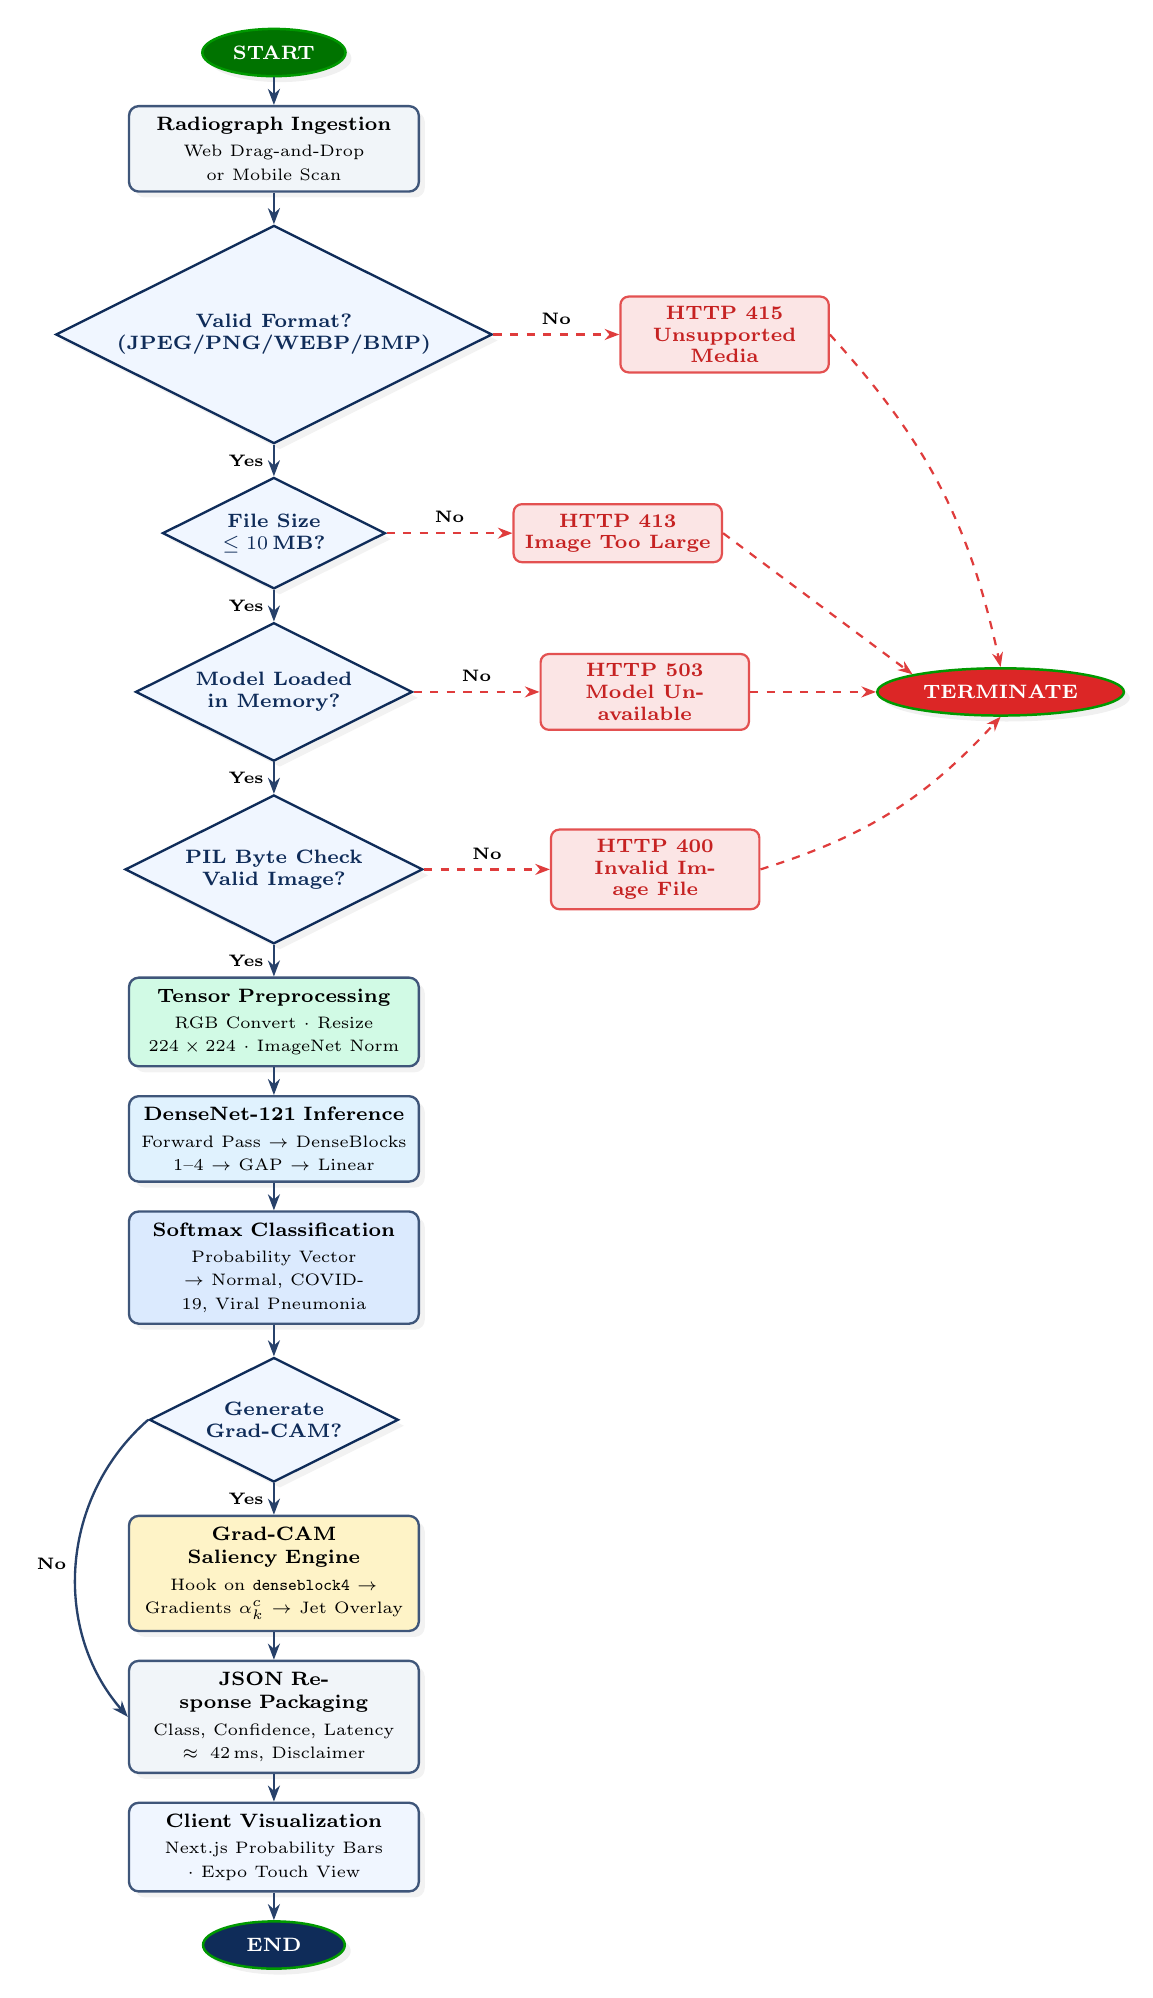
\begin{tikzpicture}[
  x=1cm, y=1cm,
  font=\sffamily,
  startend/.style={
    ellipse, draw=green!60!black, fill=green!45!black, text=white,
    line width=0.9pt, inner sep=3.5pt, font=\fontsize{7.5}{8.5}\selectfont\bfseries,
    minimum width=1.80cm, minimum height=0.60cm, drop shadow={opacity=0.12}
  },
  procbox/.style={
    rectangle, rounded corners=3.5pt,
    draw=lavenderDark!80, fill=white, text=black,
    line width=0.85pt, inner sep=4.0pt, font=\fontsize{7.2}{8.5}\selectfont,
    minimum height=0.75cm, text width=3.40cm, align=center, drop shadow={opacity=0.10}
  },
  decision/.style={
    diamond, aspect=2.0,
    draw=prismNavy, fill=lavenderLight, text=prismNavy,
    line width=0.85pt, inner sep=2.5pt, font=\fontsize{6.8}{8.0}\selectfont\bfseries,
    align=center, drop shadow={opacity=0.10}
  },
  errorbox/.style={
    rectangle, rounded corners=3pt,
    draw=statusFail!80, fill=statusFail!12, text=statusFail!90!black,
    line width=0.80pt, inner sep=3.5pt, font=\fontsize{6.8}{7.8}\selectfont\bfseries,
    minimum height=0.65cm, text width=2.40cm, align=center
  },
  flowarr/.style={
    -{Stealth[scale=0.85]}, line width=0.85pt, draw=lavenderDark!90
  },
  failarr/.style={
    -{Stealth[scale=0.80]}, line width=0.80pt, draw=statusFail!90, dashed
  }
]

  % Central Column - Main Processing Flow
  \node[startend] (start) at (0, 11.20) {START};

  \node[procbox, fill=cInput, below=0.35cm of start] (upload) {%
    \textbf{Radiograph Ingestion}\\[1pt]
    {\fontsize{6.5}{7.5}\selectfont Web Drag-and-Drop or Mobile Scan}%
  };

  \node[decision, below=0.40cm of upload] (d_mime) {%
    Valid Format?\\(JPEG/PNG/WEBP/BMP)%
  };

  \node[decision, below=0.40cm of d_mime] (d_size) {%
    File Size\\$\le 10$\,MB?%
  };

  \node[decision, below=0.40cm of d_size] (d_model) {%
    Model Loaded\\in Memory?%
  };

  \node[decision, below=0.40cm of d_model] (d_pil) {%
    PIL Byte Check\\Valid Image?%
  };

  \node[procbox, fill=cStage1, below=0.40cm of d_pil] (preprocess) {%
    \textbf{Tensor Preprocessing}\\[1pt]
    {\fontsize{6.5}{7.5}\selectfont RGB Convert $\cdot$ Resize $224\times 224$ $\cdot$ ImageNet Norm}%
  };

  \node[procbox, fill=cStem, below=0.35cm of preprocess] (infer) {%
    \textbf{DenseNet-121 Inference}\\[1pt]
    {\fontsize{6.5}{7.5}\selectfont Forward Pass $\to$ DenseBlocks 1--4 $\to$ GAP $\to$ Linear}%
  };

  \node[procbox, fill=cHead, below=0.35cm of infer] (softmax) {%
    \textbf{Softmax Classification}\\[1pt]
    {\fontsize{6.5}{7.5}\selectfont Probability Vector $\to$ Normal, COVID-19, Viral Pneumonia}%
  };

  \node[decision, below=0.40cm of softmax] (d_gradcam) {%
    Generate\\Grad-CAM?%
  };

  \node[procbox, fill=cStage2, below=0.40cm of d_gradcam] (gradcam) {%
    \textbf{Grad-CAM Saliency Engine}\\[1pt]
    {\fontsize{6.5}{7.5}\selectfont Hook on \texttt{denseblock4} $\to$ Gradients $\alpha_k^c$ $\to$ Jet Overlay}%
  };

  \node[procbox, fill=cInput, below=0.35cm of gradcam] (respond) {%
    \textbf{JSON Response Packaging}\\[1pt]
    {\fontsize{6.5}{7.5}\selectfont Class, Confidence, Latency $\approx 42$\,ms, Disclaimer}%
  };

  \node[procbox, fill=lavenderLight, below=0.35cm of respond] (render) {%
    \textbf{Client Visualization}\\[1pt]
    {\fontsize{6.5}{7.5}\selectfont Next.js Probability Bars $\cdot$ Expo Touch View}%
  };

  \node[startend, fill=lavenderDark, below=0.35cm of render] (end) {END};

  % Error Column (Right Side)
  \node[errorbox, right=1.60cm of d_mime] (e_mime) {HTTP 415\\Unsupported Media};
  \node[errorbox, right=1.60cm of d_size] (e_size) {HTTP 413\\Image Too Large};
  \node[errorbox, right=1.60cm of d_model] (e_model) {HTTP 503\\Model Unavailable};
  \node[errorbox, right=1.60cm of d_pil] (e_pil) {HTTP 400\\Invalid Image File};

  % Downward Connections
  \draw[flowarr] (start) -- (upload);
  \draw[flowarr] (upload) -- (d_mime);
  \draw[flowarr] (d_mime) -- node[left, font=\fontsize{6.5}{7.5}\selectfont\bfseries]{Yes} (d_size);
  \draw[flowarr] (d_size) -- node[left, font=\fontsize{6.5}{7.5}\selectfont\bfseries]{Yes} (d_model);
  \draw[flowarr] (d_model) -- node[left, font=\fontsize{6.5}{7.5}\selectfont\bfseries]{Yes} (d_pil);
  \draw[flowarr] (d_pil) -- node[left, font=\fontsize{6.5}{7.5}\selectfont\bfseries]{Yes} (preprocess);
  \draw[flowarr] (preprocess) -- (infer);
  \draw[flowarr] (infer) -- (softmax);
  \draw[flowarr] (softmax) -- (d_gradcam);
  \draw[flowarr] (d_gradcam) -- node[left, font=\fontsize{6.5}{7.5}\selectfont\bfseries]{Yes} (gradcam);
  \draw[flowarr] (gradcam) -- (respond);
  \draw[flowarr] (respond) -- (render);
  \draw[flowarr] (render) -- (end);

  % Branch around Grad-CAM when No
  \draw[flowarr] (d_gradcam.west) to[bend right=45] node[left, font=\fontsize{6.5}{7.5}\selectfont\bfseries]{No} (respond.west);

  % Error Branches
  \draw[failarr] (d_mime) -- node[above, font=\fontsize{6.5}{7.5}\selectfont\bfseries]{No} (e_mime);
  \draw[failarr] (d_size) -- node[above, font=\fontsize{6.5}{7.5}\selectfont\bfseries]{No} (e_size);
  \draw[failarr] (d_model) -- node[above, font=\fontsize{6.5}{7.5}\selectfont\bfseries]{No} (e_model);
  \draw[failarr] (d_pil) -- node[above, font=\fontsize{6.5}{7.5}\selectfont\bfseries]{No} (e_pil);

  % Terminate Error paths to common error end
  \node[startend, fill=statusFail, right=1.60cm of e_model] (err_end) {TERMINATE};
  \draw[failarr] (e_mime.east) to[bend left=15] (err_end.north);
  \draw[failarr] (e_size.east) -- (err_end.north west);
  \draw[failarr] (e_model.east) -- (err_end.west);
  \draw[failarr] (e_pil.east) to[bend right=15] (err_end.south);

\end{tikzpicture}
\end{document}
